\section{Краткая информация об истории развития региона}

История Башкортостана в составе России началась во времена правления Ивана Грозного. Европейская часть территорий была присоединена к России к 1557 году, присоединение периферийных земель завершилось к середине XVII века. Во второй половине XVII века из-за внутренней политики России разгораются массовые восстания. Непосредственное участие коренное население приняло в Крестьянской войне 1773-1775 гг. Массовые выступления, их жесткое подавление отрицательно повлияли на развитие края и его производительные силы, а также на численность населения. 

\begin{wrapfigure}{r}{0.5\linewidth}
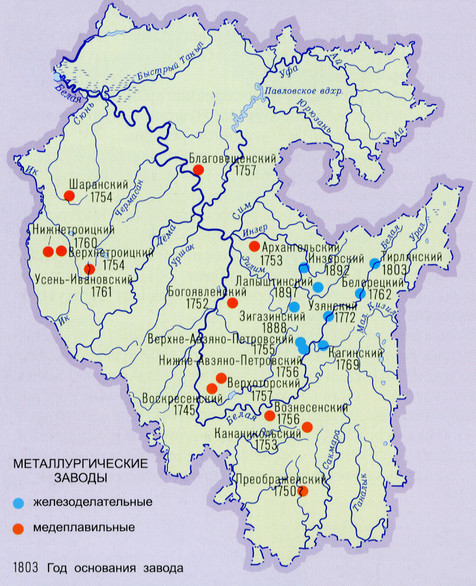
\includegraphics[width=1\linewidth]{pics/sasha/factories_18-19} 
\caption{Металлургические заводы, XVIII-ХIХ вв.}
\end{wrapfigure}
Со второй половины XVIII века начинают сооружаться заводы. В первой половине ХIХ века по всей России развиваются рыночные отношения, а феодально-крепостническая система терпит кризис. После революций 1917 года в Башкортостане началось движение за создание национальной республики в составе федеративной России. 20 марта 1919 г. была создана Башкирская Автономная Советская Республика. 

Во время Гражданской войны экономика республики претерпела серьезный урон: объем производства промышленности упал на 70\% и восстановился лишь к 1926 году. В 1921-22 гг. в следствие массового голода численность населения в Башкортостане сократилась на 22\%, в два раза уменьшилось число посевных площадей. Тем не менее аграрный сектор по-прежнему занимал ведущую роль. 

В 1920-30-е годы начался рост промышленного производства (темпы роста в \%: в 1913 — 1,0; в 1940 — 10; в 1950 — 41; в 1960—186; в 1970—478; в 1980—983; в 1990—1221). За годы 1-й пятилетки в БАССР были реконструированы Белорецкие заводы, которые впоследствии стали крупнейшими предприятиями СССР по производству высококачественной стали, было построено свыше 30 новых заводов, фабрик и электростанций. Республика стала аграрно-индустриальной: в 1932 году 50\% валовой продукции шло от промышленности. Промышленно-производственные фонды выросли в 2,5 раза, выпуск продукции – в 2,3 раза. В следующие пятилетки было построено более 70 производственных объектов. В 40-80-е годы шло индустриальное освоение богатых природных ресурсов региона. Всего за это время промышленное производство увеличилось в 81 раз.

В 1929 году геологоразведка доложила о возможных больших залежах нефти в районе современного Ишимбая. Началась разработка первого нефтяного месторождения. Начало нефтедобывающей промышленности Башкортостана было положено в 1932 году,  когда одна из скважин дала фонтан нефти. Первый нефтеперерабатывающий завод был основан в 1936 году.

1941 - 1945 гг. – Великая Отечественная война. Башкортостан стал одним из важнейших регионов перебазирования промышленности страны. В 1941—1942 годах в республику было эвакуировано около ста заводов и фабрик. Промышленность была перестроена на выпуск военной и оборонной продукции. Производительность труда в промышленности возросла в 2, в машиностроении – в 3 раза, увеличилась добыча металлов и металлообработка. В 1943 г. было открыто Кинзябулатовское нефтяное месторождение, и переработка нефти возросла в 1,5 раза.

К 1946 году промышленность БАССР возвращается на мирный лад. Развиваются и разрабатываются месторождения. Республика становится ведущим регионом по нефтепереработке, а по добыче нефти занимает второе место в СССР. Одной из ведущих отраслей региона становится химическая промышленность. Развиваются горнорудная и машиностроительная отрасли, химическая отрасль становится одной из ведущих региона. В 1966-1980 гг. в БАССР были запущены 832 предприятия. За 15 лет основные промышленно-производственные фонды выросли в 2,8 раза, а выпуск продукции – в 2,4 раза. 

\begin{figure}[h!]
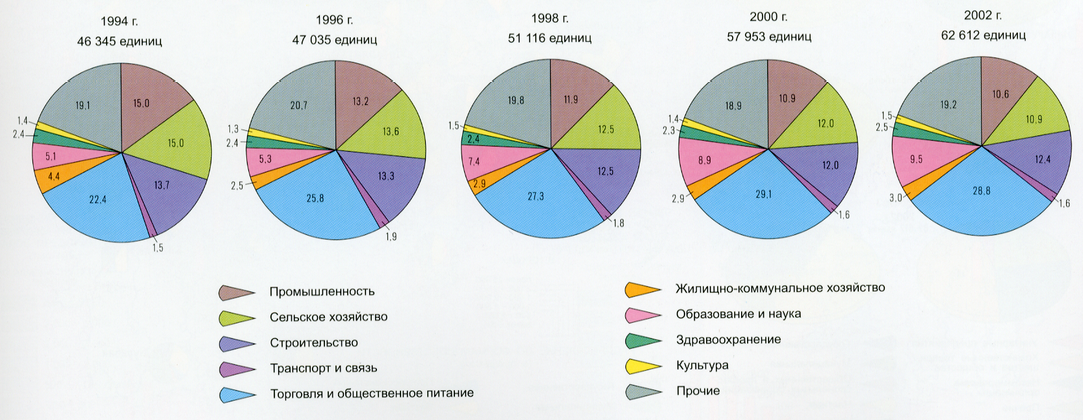
\includegraphics[width=1\linewidth]{pics/sasha/industries} 
\caption{Распределение предприятий и организаций Башкортостана по отраслям (\%)}
\end{figure}

Современная Республика Башкортостан была образована 11 октября 1990 года (Декларация о государственном суверенитете). 

К 1990-м годам 97\% заводов, шахт и фабрик на территории Башкортостана находились в собственности союзных, республиканских министерств и ведомств. С 1992 года началось акционирование предприятий. В настоящее время масштабную инвестиционную деятельность в Башкортостане ведёт ПАО «Газпром». 

\section{Отраслевая и территориальная структура экономики}

\begin{wrapfigure}{l}{0.4\linewidth}
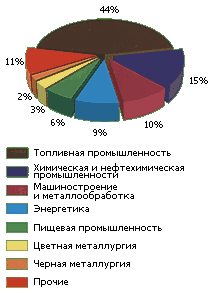
\includegraphics[width=1\linewidth]{pics/sasha/promstruct}
\caption{Отраслевая структура промышленности}
\end{wrapfigure}
Центрами промышленного производства Башкортостана являются города Уфа, Стерлитамак, Салават, Ишимбай и Нефтекамск. На предприятиях этих городов производится более половины объёма всей промышленной продукции Башкортостана. (См. \ref{fig:economics})

\subsection{Нефтедобыча и нефтехимическая промышленность}

В республике разведано 191 месторождение нефти и газа, из них в разработке находится 161 месторождение. Ведущее нефтегазодобывающее предприятие Башкирии — ПАО «Акционерная нефтяная компания „Башнефть“», на долю которого приходится более 98\% объёма нефтедобычи и практически весь объём добываемого газа.

Нефтехимическая промышленность представлена производствами автомобильного бензина, керосина, дизельного топлива, минеральных удобрений. В Башкортастане производят половину объёма кальцинированной соды, бутиловых и изобутиловых спиртов России, более четверти химических средств защиты растений, пятую часть каустической соды, шестую часть автомобильного бензина, дизельного топлива и синтетических каучуков, седьмую часть синтетических смол и пластмасс, восьмую часть полиэтилена, десятую часть топочного мазута. В регионе находится крупнейшее в России предприятие по производству катализаторов. 

Ведущие предприятия:
\begin{itemize}
\item г. Уфа: «Башнефть-Уфанефтехим», «Башнефть-УНПЗ» и «Башнефть-Новойл»; ОАО «Уфаоргсинтез»
\item г. Салават: ОАО «Газпром нефтехим Салават»
\item г. Стерлитамак: ОАО «Стерлитамакский нефтехимический завод»; ОАО «Башкирская содовая компания»
\end{itemize}

В 2019-2021 годах планируется увеличение промпроизводства (см. \href{https://neftegaz.ru/news/finance/197497-rost-promproizvodstva-v-2019-2021-gg-v-respublike-bashkortostan-obespechat-neftekhimiya-i-aviaprom/}{статью}).

\subsection{Машиностроение и металлообработка}

Машиностроительный комплекс представлен около 300 крупными и средних предприятиями. Развиты электротехническая промышленность, производство оборудования для металлургических производств и сельского хозяйства, приборо- и станкостроение. Крупнейшие производства:
\begin{itemize}
\item оборудования для предприятий нефтедобычи, нефте- и газопереработки, химии и нефтехимии: г. Ишимбай (ОАО «Ишимбайский машиностроительный завод», ООО «Идель Нефтемаш») и г. Салават (ОАО «Салаватнефтемаш»)
\item вертолетов: г. Кумертау (ОАО «Кумертауское авиационное производственное предприятие»)
\item автобусов: г. Нефтекамск (ОАО «Нефтекамский автозавод»)
\item троллейбусов: г. Уфа (ОАО «Башкирский троллейбусный завод»)
\item вездеходов: г. Ишимбай (АО «Машиностроительная компания „Витязь“»)
\end{itemize}

\subsection{Пищевая промышленность}

Пищевая промышленность Башкортастана представлена всеми необходимыми для жизни продуктами питания: мясной, молочной, кондитерской, ликёроводочной, пивоваренной, чайной продукциями. Крупнейшие предприятия: ОАО «Башспирт» (Стерлитамакский спиртоводочный комбинат, Уфимский вино-водочный завод), Карламанский молочно-консервный комбинат, Уфимский мясоконсервный комбинат, Мелеузовский МКК, Белорецкий рыбозавод и тд.

\subsection{Энергетика}

На топливно-энергетический комплекс (ТЭК) приходится 50\% общерегионального объёма отгруженной продукции, 70\% полученной прибыли, 40\% поступлений в консолидированный бюджет республики, более 30\% инвестиций в основной капитал и 80\% валютных поступлений. ТЭК Башкортостана является также значительной составной частью национальной экономики России.

Башкортостан обладает развитой энергетической базой и обеспечивает потребность в электро- и теплоэнергии на региональном уровне. Системообразующее предприятие отрасли — ОАО «Башкирская электросетевая компания», дающее более 90\% электрической энергии и около 50\% тепловой энергии региона. В настоящее время в республике работает 31 электростанция (см. \href{https://energybase.ru/region/respublika-bashkortostan}{energybase.ru}).

\subsubsection{Перспективы отрасли}

В силу географического положения и климатических особенностей Башкортостан обладает одними из наиболее благоприятных условий для солнечной энергетики среди российских регионов. Уровень инсоляции соответствует показателям южных районов Европы. Количество солнечных дней в Башкортостане составляет около 260 (в Сочи — 190, в Москве — 114). В настоящее время в эксплуатации находятся 3 солнечные электростанции и идет дальнейшее развитие в данном направлении. 

Вблизи города Агидель расположена недостроенная Башкирская АЭС. Проектная мощность составляла 4000 МВт. Возобновление строительства возможно после 2020 года в случае возникновения необходимости в дополнительной выработке электроэнергии.

\subsection{Сельское хозяйство}

\begin{wrapfigure}{l}{0.6\linewidth}
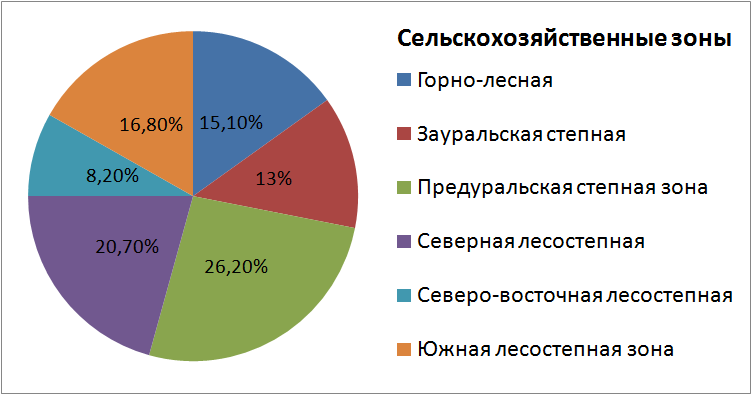
\includegraphics[width=1\linewidth]{pics/sasha/zones}
\end{wrapfigure}

Сельское хозяйство региона представлено в основном зерново-животноводческими направлениями. Выращиваются пшеница, рожь, овёс, ячмень (зерновые культуры) и сахарная свёкла, подсолнечник (технические культуры), гречиха. В республике развито мясо-молочное животноводство, мясо-шёрстное овцеводство, птицеводство, коневодство, кумысоделие и пчеловодство. Широко известен башкирский мёд.

В 2015 году Башкортостан занимал первое место в России по поголовью крупного рогатого скота, лошадей, производству мёда и молока, второе место — по производству картофеля, третье — производству мяса, пятое и шестое — поголовью свиней, овец и коз соответственно, восьмое — производству яиц, одиннадцатое — по производству зерна. Развивается частный сектор: более трети валовой продукции сельского хозяйства приходится на личные подсобные и крестьянские (фермерские) хозяйства. Кроме того, в регионе достаточно водных ресурсов для развития рыбоводства.

\subsection{Транспорт} 

Из-за широкого развития грузоемких отраслей промышленности транспортная отрасль имеет повышенное значение (\href{https://ru.wikipedia.org/?oldid=99559170}{ru.wikipedia.org}). Транспортная сеть Башкортостана обеспечивает не только внутриреспубликанские, но и мощные транзитные потоки грузов и пассажиров между азиатской и европейской частями России. Важное значение имеют железная дорога Самара-Уфа-Челябинск, многониточные трубопроводы, высоковольтные ЛЭП Поволжье-Урал и автомагистрали Самара-Уфа-Челябинск.

Особенности:
\begin{enumerate}
\item Высокий удельный вес в перевозках имеет трубопроводный транспорт.
\item Ведущее место в транспортном обслуживании многоотраслевого хозяйства Башкортостана принадлежит железным дорогам.
\item Объем перевозок грузов транспортом общего пользования (за исключением трубопроводного) в Башкортастане в целом сокращается (как следствие общего спада производства и разрыва межрегиональных и межгосударственных хозяйственных связей).
\item В перевозках пассажиров резкое преобладание принадлежит автомобильному транспорту.
\end{enumerate}

\subsection{Туризм}

Среди отраслей экономики Башкортостана существенную роль играет туризм. Есть перспективы развития туризма как индустрии, приносящей устойчивый доход. Туристские ресурсы республики: памятники культуры и искусства городов Уфы, Стерлитамака, Ишимбая, Салавата и др.; около 300 карстовых пещер; 600 рек, с крупнейшей рекой Белой; 800 озёр; хребты Уральских гор; три государственных заповедника (Шульган-Таш, Башкирский заповедник, Южно-Уральский заповедник) и национальный природный парк («Башкирия»). В республике представлены различные маршруты: доступные и спортивные сплавы по рекам, горные одно- и многодневные маршруты, велотреки, природные скалы для скалолазания, удобные тропы для конных прогулок. На озёрах и водохранилищах действуют десятки туристических баз и санаториев. Есть известные объекты для паломничества православных верующих.

\begin{figure}[h!]
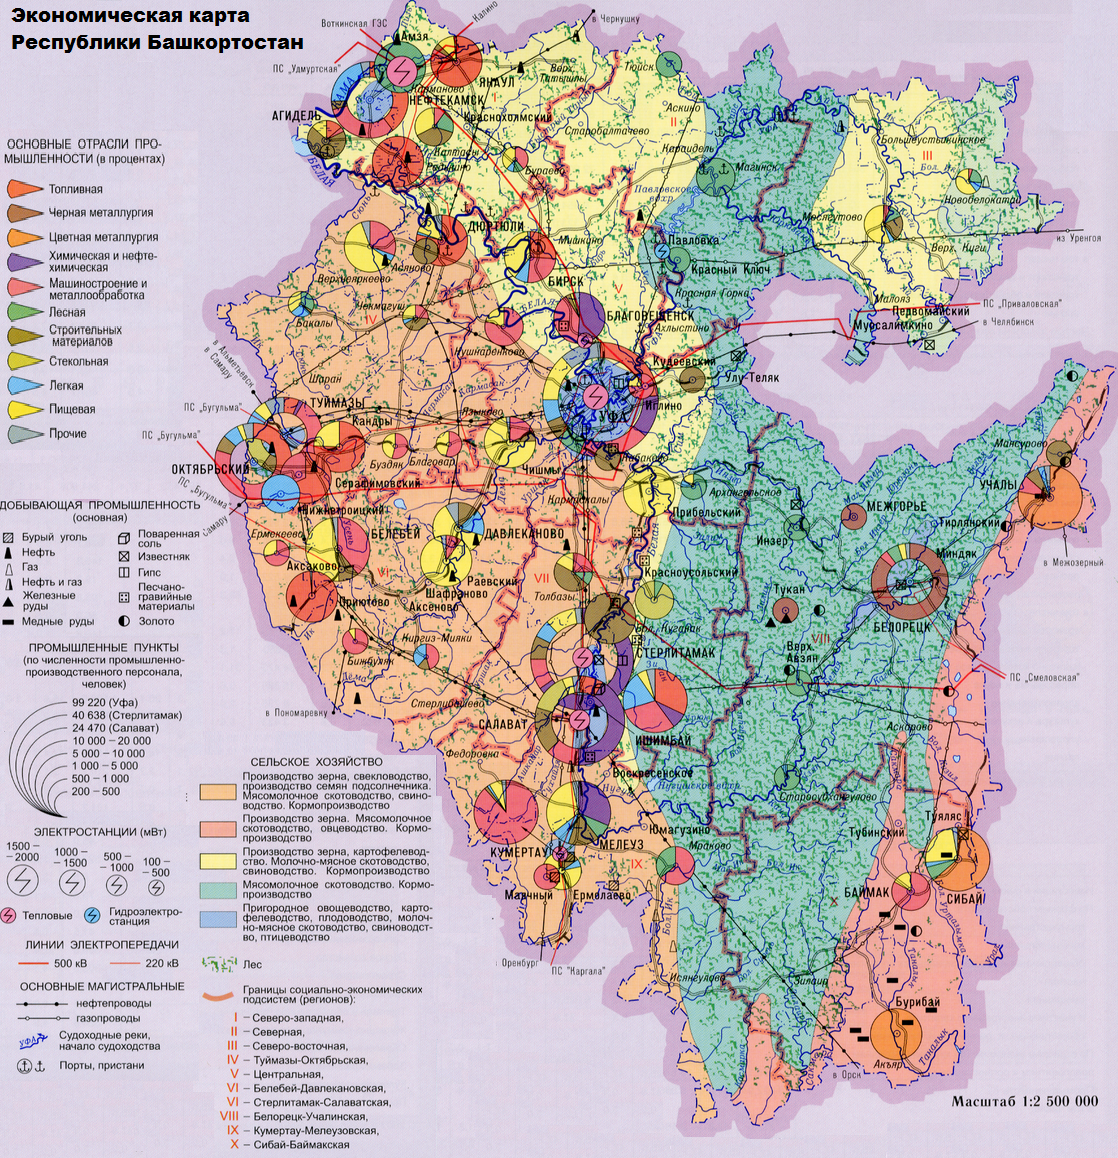
\includegraphics[width=1\linewidth]{pics/sasha/economics}
\caption{Экономическая карта республики Башкоторстан)}\label{fig:economics}
\end{figure}

